%% Pompe à main : dessin d'ensemble en coupe, pièces numérotées (0 corps, 1 levier, 2 bielle,
%% 3 piston, 4 axe du levier, 5 joint du piston).
\documentclass[tikz,border=4pt]{standalone}
\usepackage{liaisons}
%% Dessin d'ensemble simplifié de la pompe à main (coupe). Inclus par mecanisme-pompe-a-main-dessin.tex
%% et mecanisme-pompe-a-main-classes.tex, qui définissent \piece{numéro}{chemin} (une mise en forme par
%% pièce) et \pplabels (étiquettes : numéros de pièces ou classes d'équivalence).
%% Repère : x horizontal, y vertical (axe du cylindre). Cotes en cm.
%% Points : O (4.15, 7.25) pivot levier/corps ; A (2.3, 7.25) pivot levier/bielle ; B (2.3, 5.1) pivot bielle/piston.
\newcommand\pompeamain{%
  \begin{scope}[line width=0.6pt, line join=round]
    % 0 : corps de pompe (coupé) — parois du cylindre, fond, bec verseur, chape du levier
    \piece{0}{(1.35,0.4) rectangle (1.8,4.7)}
    \piece{0}{(2.8,0.4) rectangle (3.25,4.7)}
    \piece{0}{(1.15,0.0) rectangle (3.45,0.4)}
    \piece{0}{(1.35,3.55) -- (0.3,3.55) -- (0.3,2.75) -- (0.75,2.75) -- (0.75,3.1) -- (1.35,3.1) -- cycle}
    \piece{0}{(2.8,4.7) -- (4.6,4.7) -- (4.6,7.45) -- (3.7,7.45) -- (3.7,5.2) -- (2.8,5.2) -- cycle}
    % axe du cylindre
    \draw[dash pattern=on 6pt off 2pt on 1pt off 2pt, line width=0.4pt] (2.3,-0.3) -- (2.3,5.9);
    % 3 : piston (tige + tête) — 5 : joint (garniture)
    \piece{3}{(2.1,1.9) rectangle (2.5,5.35)}
    \piece{3}{(1.8,1.1) rectangle (2.8,1.9)}
    \piece{5}{(1.8,1.9) rectangle (2.8,2.12)}
    % 1 : levier (barre + poignée)
    \piece{1}{[rounded corners=3pt] (1.75,7.02) rectangle (6.4,7.48)}
    \piece{1}{[rounded corners=5pt] (6.1,6.75) rectangle (6.95,7.75)}
    % 2 : bielle (corps + deux têtes)
    \piece{2}{(2.16,5.1) rectangle (2.44,7.25)}
    \piece{2}{(2.3,7.25) circle (0.32)}
    \piece{2}{(2.3,5.1) circle (0.32)}
    % 4 : axe du levier (chassé dans la chape du corps)
    \piece{4}{(4.15,7.25) circle (0.2)}
    % axes des pivots A et B
    \foreach \p in {(2.3,7.25), (2.3,5.1)} { \draw[fill=white, line width=0.5pt] \p circle (0.09); }
    % points caractéristiques
    \node[fill=white, inner sep=1pt, font=\small] at (1.62,7.25) {A};
    \node[fill=white, inner sep=1pt, font=\small] at (1.62,5.1) {B};
    \node[fill=white, inner sep=1pt, font=\small] at (4.15,6.6) {O};
    \pplabels
  \end{scope}}

\begin{document}
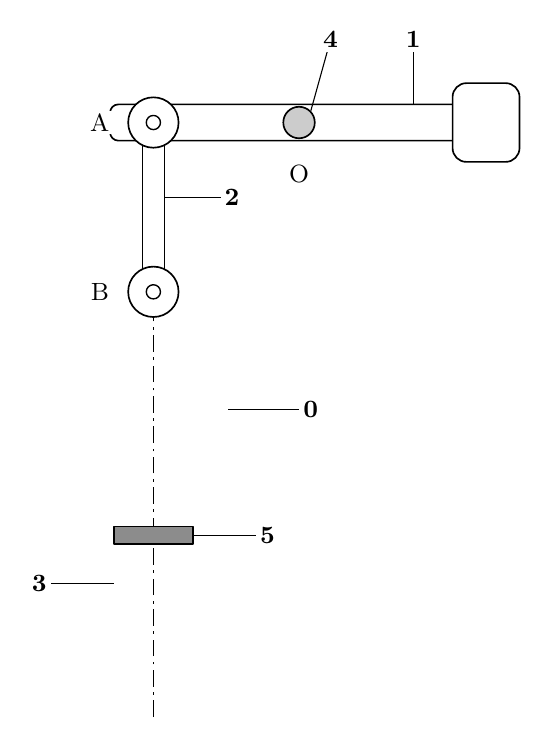
\begin{tikzpicture}[x=1cm,y=1cm]
\newcommand\piece[2]{\ifcase#1\relax
  \hachures{#2}                                                        % 0 corps (coupé)
  \or \draw[line width=0.6pt, line join=round, fill=white] #2;         % 1 levier
  \or \draw[line width=0.6pt, line join=round, fill=white] #2;         % 2 bielle
  \or \hachuresb{#2}                                                   % 3 piston (coupé)
  \or \draw[line width=0.6pt, line join=round, fill=black!20] #2;      % 4 axe
  \or \draw[line width=0.6pt, line join=round, fill=black!45] #2;      % 5 joint
  \fi}
\newcommand\pplabels{%
  \foreach \n/\pt/\lab in {0/{(3.25,3.6)}/{(4.3,3.6)}, 1/{(5.6,7.48)}/{(5.6,8.3)}, 2/{(2.44,6.3)}/{(3.3,6.3)},
                           3/{(1.8,1.4)}/{(0.85,1.4)}, 4/{(4.3,7.4)}/{(4.55,8.3)}, 5/{(2.8,2.0)}/{(3.75,2.0)}} {
    \draw[line width=0.4pt] \pt -- \lab;
    \node[fill=white, inner sep=1.5pt, font=\small\bfseries] at \lab {\n};
  }}
\pompeamain
\repere{(5.4,0.9)}{x}{y}{1}
\end{tikzpicture}
\end{document}
